%!TEX root = ../thesis.tex
%*******************************************************************************
%*********************************** Expirements *****************************
%*******************************************************************************

\chapter{Year 1 Activity}  %Title of the Year 1 Activity

\ifpdf
    \graphicspath{{Year1Activity/Figs/Raster/}{Year1Activity/Figs/PDF/}{Year1Activity/Figs/}}
\else
    \graphicspath{{Year1Activity/Figs/}{Year1Activity/Figs/}}
\fi

This is section will be split into the timeline of activities of year 1.

\subsection{Literature review year 1}
Background reading was conducted about the topics of Unikernels, Multi-Kernels and 
TAG based architecture as mentioned in this following report. 

\subsection{Poster SISCA PhD Conference}
The PhD symposium was held in in Glasgow Caledonian University for 2 days. A poster 
by the title "Benchmarking Unikernels with distributed map reduce"\cite{Sisca2022Poster}. The
objective for attending this conference was to socialize with other PhD students 
in Scotland by also presenting one of the plans of the initial experiments. 

Submission type:
\begin{enumerate}
    \item Poster: "Benchmarking Unikernels with distributed map reduce"\cite{Sisca2022Poster}
\end{enumerate}

\subsection{Europar PhD symposium and poster session}
The Europar PhD conference was held in the university of Glasgow. The title 
of the symposium paper being "Benchmarking Parallelism in Unikernels"\cite{Europar2022Paper}. This 
is expected to be published in springer proceeding of Europar 2022. 

Submission type:
\begin{enumerate}
    \item Poster: "Benchmarking Parallelism in Unikernels"\cite{Europar2022Poster}
    \item PhD Symposium paper: "Benchmarking Parallelism in Unikernels"\cite{Europar2022Paper}
\end{enumerate}

\subsubsection{Submitted paper abstract}
Virtualisation technologies are widely used in Cloud computing
infrastructures, because they can be provisioned cheaply and quickly
to meet demand. The common approaches are either to package a
Operating System (OS) as a Virtual Machine, or to containerise
software with an OS kernel. An emerging alternative are unikernels,
which are customised kernels to support just one application.
% why is it interesting
Unikernels are lightweight and an applications has sole use of the
kernel, which offers potential for fast, resource efficient and
secure execution. For these reasons, unikernels may be idea for
parallel computing in the Cloud. However, the parallel performance
of unikernel-based Cloud applications has not been extensively
studied.
% what is this paper's solution
This paper presents an evaluation of the OSv unikernel using a
parallelised Mandelbrot benchmark, comparing with Docker and a
monolithic VM for runtime, parallel speedups and boot-up time. OSv
has the fastest boot-up time, and is comparable with the parallel
speedups of Docker and the monolithic VM.


\begin{figure}[htbp!] 
    \centering    
    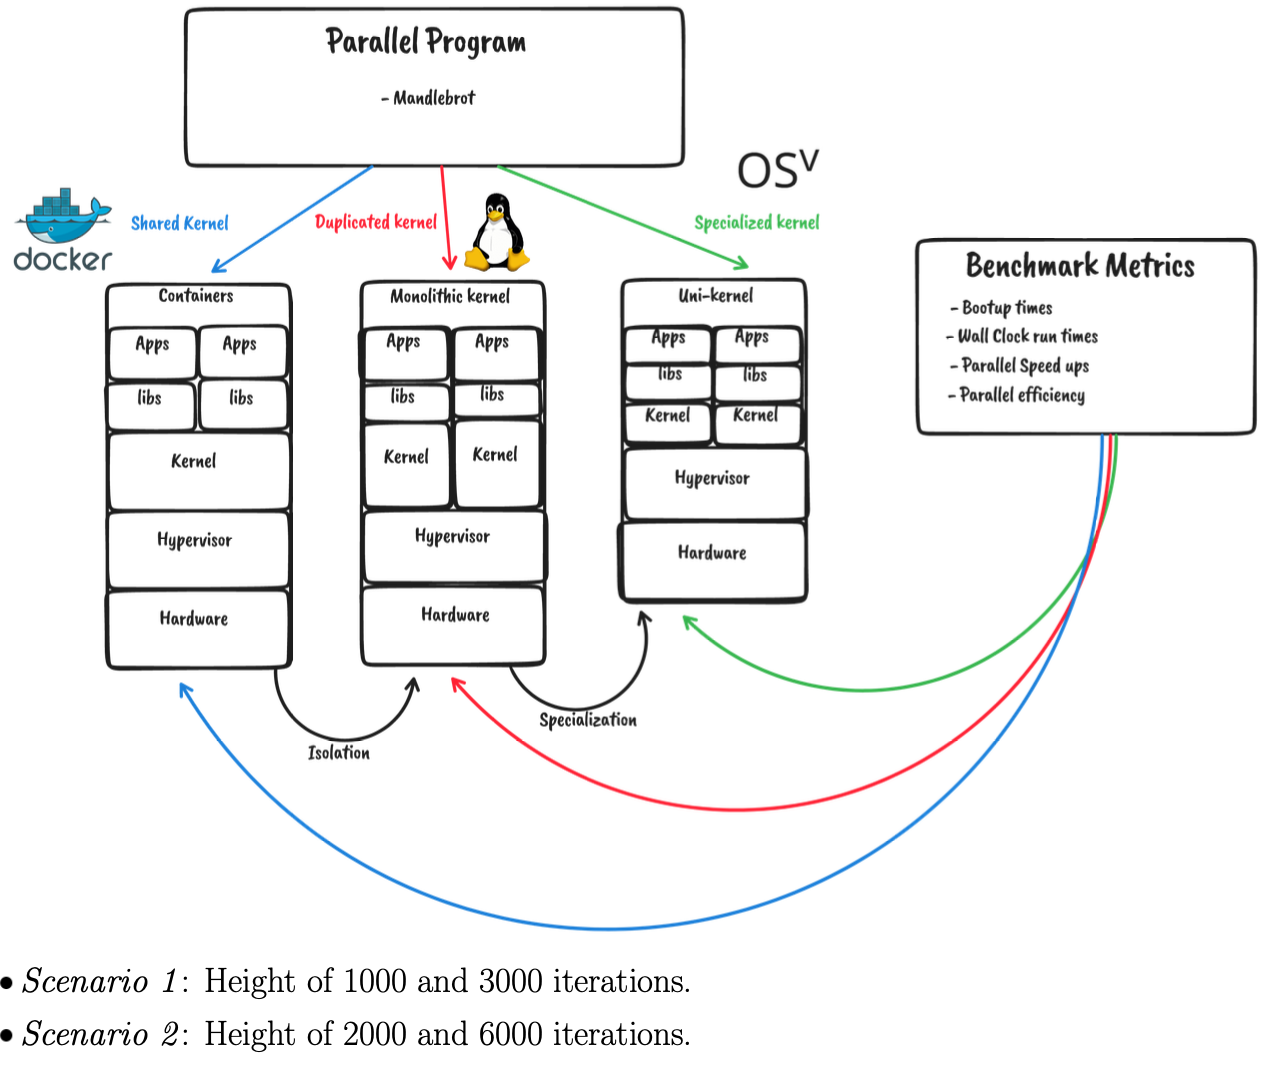
\includegraphics[width=0.6\textwidth]{madelbrot-expirment}
    \caption[Year1-Activity-Uni-kernel-activity-diagram]{Uni-kernel comparison experiment}
    \label{fig:UnikernelExpirement}
\end{figure}



